% Compile twice with XeLaTeX. All displayed figures come from numerics.py.
\documentclass[11pt,letterpaper]{article}
\usepackage[margin=.85in,headheight=14pt]{geometry}
\usepackage{fontspec}
\setmainfont{Latin Modern Roman}
\setsansfont{DejaVu Sans}[Scale=.9]
\setmonofont{DejaVu Sans Mono}[Scale=.8]
\usepackage{amsmath,amsthm,booktabs,tabularx,array}
\usepackage{unicode-math}
\setmathfont{Latin Modern Math}
\usepackage{xcolor,graphicx,caption,fancyhdr,enumitem,microtype}
\usepackage[hidelinks]{hyperref}
\definecolor{Ink}{HTML}{173756}
\definecolor{Teal}{HTML}{138477}
\definecolor{Grey}{HTML}{536475}
\hypersetup{pdftitle={A Brownian Functional and Its Predictable Compensator},pdfauthor={Eliguli Han}}
\pagestyle{fancy}\fancyhf{}
\fancyhead[L]{\small\sffamily\color{Grey} BROWNIAN FUNCTIONALS}
\fancyhead[R]{\small\sffamily\color{Grey} PROOF AND COMPUTATION}
\fancyfoot[C]{\small\thepage}
\setlength{\parindent}{0pt}\setlength{\parskip}{4pt}
\setlength{\emergencystretch}{2em}
\setlength{\abovedisplayskip}{6pt}\setlength{\belowdisplayskip}{6pt}
\setlist[enumerate]{leftmargin=1.65em,itemsep=3pt,topsep=3pt}
\captionsetup{font=small,labelfont=bf,skip=5pt}
\newtheorem{theorem}{Theorem}
\newtheorem{lemma}[theorem]{Lemma}
\newcommand{\E}{\mathbb E}
\newcommand{\Pbb}{\mathbb P}
\newcommand{\R}{\mathbb R}
\newcommand{\F}{\mathcal F}
\newcommand{\dd}{\,\mathrm d}
\newcommand{\ind}{\mathbf1}
\newcommand{\norm}[1]{\left\lVert #1\right\rVert}
\DeclareMathOperator{\Var}{Var}
\DeclareMathOperator{\Cov}{Cov}
\allowdisplaybreaks[2]
\newcommand{\SamplePaths}{8192}
\newcommand{\FineSteps}{2048}
\newcommand{\RandomSeed}{20261123}
\newcommand{\SemigroupError}{$5.551\times10^{-17}$}
\newcommand{\PrimitiveError}{$1.943\times10^{-16}$}
\newcommand{\ExpectedP}{$-0.060605968062$}
\newcommand{\ExpectedK}{$-0.060605968062$}
\newcommand{\MeanM}{$1.369\times10^{-4}$}
\newcommand{\SEMeanM}{$1.328\times10^{-3}$}
\newcommand{\CoarseError}{$0.0156212$}
\newcommand{\FineError}{$0.0028902$}
\newcommand{\ConvergenceSlope}{$0.4887$}
\newcommand{\PDEError}{$4.842\times10^{-7}$}
\newcommand{\EnergyAdaptive}{$0.0155568966$}
\newcommand{\EnergyBound}{$3.06382946$}
\newcommand{\ZMean}{0.103}

\begin{document}
\begin{center}
{\LARGE\bfseries\color{Ink} A Brownian Functional and Its\\[3pt] Predictable Compensator}\par
\vspace{5pt}
{\large Complete analytic solution of parts (a)--(d),\\Lean-checked components and numerical experiments}\par
\vspace{6pt} Eliguli Han\quad |\quad 23 November 2026
\end{center}
\vspace{3pt}\hrule\vspace{6pt}

\textbf{Abstract.}
For the recorded finite-sum payoff containing positive parts and indicator functions, we prove the backward heat equation, compute the It\^o decomposition of an integrated Brownian functional, identify its predictable finite-variation compensator, and establish a square-integrable martingale on the closed interval $[0,T]$. We retain the spatial lower-endpoint term, justify every growth and terminal-time estimate, and give an explicit Gaussian formula suitable for computation. Independent quadrature and nested Brownian simulations illustrate the result.

\textbf{Formal verification status.}
The accompanying Lean sources compile in Lean 4.36.0 with the pinned Mathlib revision recorded in the verification ledger. They verify the original payoff's measurability and growth bound, actual heat-kernel derivatives, spatial primitive derivatives, integration by parts, the moment-majorant time integral, Brownian finite moments, and a conditional-payoff martingale. The complete theorem identifying $P-K$ as the stochastic integral, including its closed-interval martingale property, remains an open formalization obligation. The mathematical proof below is complete; the Lean artifact has explicitly delimited coverage.

\textbf{Public verification links.}
\href{https://github.com/Eliguli712/brownian_motion/blob/73a1d2ff4f3125264fe3d2e9d1daa013fd31582e/compensator/Brownian_Compensator_Verified_Components.lean}{Permanent Lean source},
\href{https://github.com/Eliguli712/brownian_motion/blob/73a1d2ff4f3125264fe3d2e9d1daa013fd31582e/compensator/README.md}{reproduction instructions}, and
\href{https://github.com/Eliguli712/brownian_motion/actions/runs/45158953034}{GitHub Actions verification record}
are public. Figure~\ref{fig:proofmap} maps the proof dependencies and verification boundary.


\section{Recorded problem and precise hypotheses}
This is the problem recorded in \texttt{Brownian\_Compensator\_Full\_Problem\_Solutions.pdf}, saved on 29 October 2026. Its four parts are labeled (a)--(d). The source is a previously saved solution document.

Let $(\Omega,\F,(\F_t)_{0\le t\le T},\Pbb)$ satisfy the usual conditions, let $T>0$, and let $W$ be a standard Brownian motion \emph{relative to this filtration}. Thus $W_t-W_s$ is independent of $\F_s$ for $s\le t$. Fix $n\ge2$ and $a_1,\ldots,a_n\in\R$. Write $u^+=\max(u,0)$ and define
\begin{equation}\label{eq:g}
g(x)=\frac1{n^2}\sum_{i,j=1}^n
\left[-\frac14(a_i+x)^++\frac12(a_j-a_i)^+
-\frac14\ind_{\{a_i+a_j+2x<1\}}\right].
\end{equation}
For $0\le t<T$, set
\begin{equation}\label{eq:defS}
S(t,x)=\E[g(x+W_T-W_t)],\qquad
P_t=\int_0^{W_t}rS(t,r)\dd r.
\end{equation}
All spatial integrals are \emph{oriented}: $\int_0^x=-\int_x^0$ when $x<0$.

\begin{enumerate}[label=\textbf{(\alph*)}]
\item Prove $S_t+\tfrac12S_{xx}=0$ for $t<T$.
\item Derive the semimartingale decomposition of $P$ using It\^o's formula.
\item Find a predictable process $b$ for which $M_t=P_t-\int_0^t b_s\dd s$ is a martingale.
\item Prove the required integrability and extend the conclusion to $t=T$.
\end{enumerate}
The additional compensator question asks for the normalized predictable finite-variation process $K$ in $P=K+M$.

\begin{theorem}\label{thm:main}
The process $P$ has a continuous extension to $T$ given by
\begin{equation}\label{eq:PT}
P_T=\int_0^{W_T}rg(r)\dd r.
\end{equation}
Its predictable finite-variation compensator, normalized by $K_0=0$, is
\begin{equation}\label{eq:K}
\boxed{K_t=\int_0^t\left[S(s,W_s)-\frac12S(s,0)\right]\dd s.}
\end{equation}
For every $0\le t\le T$, the decomposition is
\begin{equation}\label{eq:main}
\boxed{P_t=K_t+M_t,\qquad M_t=\int_0^tW_sS(s,W_s)\dd W_s.}
\end{equation}
Here $M$ is a continuous square-integrable martingale with
\begin{equation}\label{eq:qv}
\E[M_t\mid\F_s]=M_s\quad(s\le t),\qquad
\langle M\rangle_t=\int_0^tW_s^2S(s,W_s)^2\dd s.
\end{equation}
\end{theorem}

\section{The original payoff: measurability, growth and closed form}
Put $c_{ij}=(1-a_i-a_j)/2$ and
\begin{equation}\label{eq:constants}
D=\frac1{2n^2}\sum_{i,j}(a_j-a_i)^+,
\qquad
A=\frac1{4n}\sum_i|a_i|+D+\frac14.
\end{equation}
The indicator in \eqref{eq:g} equals $\ind_{\{x<c_{ij}\}}$, hence
\begin{equation}\label{eq:grewrite}
g(x)=-\frac1{4n}\sum_i(a_i+x)^++D
-\frac1{4n^2}\sum_{i,j}\ind_{\{x<c_{ij}\}}.
\end{equation}
Every term is Borel measurable. The positive-part terms are continuous and the indicator terms have a finite set of possible jump locations. Since $(a_i+x)^+\le|a_i|+|x|$ and each indicator is between zero and one,
\begin{equation}\label{eq:growthg}
\boxed{|g(x)|\le A+\frac14|x|.}
\end{equation}

Let $\varphi(z)=(2\pi)^{-1/2}e^{-z^2/2}$ and $\Phi(z)=\int_{-\infty}^z\varphi(u)\dd u$.
For $\sigma>0$, direct integration yields
\begin{align}
H_\sigma(z)&:=\E[(z+\sigma Z)^+]
=\int_{-z/\sigma}^{\infty}(z+\sigma u)\varphi(u)\dd u\notag\\
&=z\Phi(z/\sigma)+\sigma\varphi(z/\sigma),\quad Z\sim N(0,1),\label{eq:H}
\end{align}
using $\varphi'(u)=-u\varphi(u)$ and Gaussian symmetry. With $\sigma=\sqrt{T-t}$,
\begin{equation}\label{eq:Sexplicit}
\boxed{
S(t,x)=-\frac1{4n}\sum_iH_\sigma(a_i+x)+D
-\frac1{4n^2}\sum_{i,j}\Phi\!\left(\frac{c_{ij}-x}{\sigma}\right).}
\end{equation}
This finite formula handles the original nonsmooth payoff directly.

\subsection*{Conditional-expectation interpretation}
The independent Brownian increment is $\sqrt{T-t}\,Z$ in distribution, independently of $\F_t$. Therefore
\begin{equation}\label{eq:StCE}
S(t,W_t)=\E[g(W_T)\mid\F_t].
\end{equation}
The growth bound makes $g(W_T)$ integrable, and in fact square-integrable. The tower property proves that $S(t,W_t)$ itself is a martingale. The compensator theorem concerns the further integral functional $P_t$.

\section{Part (a): the backward heat equation}
Two complementary computations establish the analytic step.

\subsection*{Direct differentiation of the finite formula}
Set $v=T-t$, $\sigma=\sqrt v$, $z_i=(a_i+x)/\sigma$ and $q_{ij}=(c_{ij}-x)/\sigma$. The two smoothing building blocks obey
\begin{align}
\partial_xH_\sigma(a_i+x)&=\Phi(z_i),&
\partial_{xx}H_\sigma(a_i+x)&=\frac{\varphi(z_i)}\sigma,&
\partial_tH_\sigma(a_i+x)&=-\frac{\varphi(z_i)}{2\sigma},\label{eq:callDerivs}\\
\partial_x\Phi(q_{ij})&=-\frac{\varphi(q_{ij})}\sigma,&
\partial_{xx}\Phi(q_{ij})&=-\frac{q_{ij}\varphi(q_{ij})}{v},&
\partial_t\Phi(q_{ij})&=\frac{q_{ij}\varphi(q_{ij})}{2v}.\label{eq:digitalDerivs}
\end{align}
For example, $\partial_tq_{ij}=q_{ij}/(2v)$ and $\partial_xq_{ij}=-1/\sigma$, which give the second line by the chain rule. Each summand in \eqref{eq:Sexplicit} satisfies the backward heat equation, and the constant $D$ does as well. Finite summation proves
\begin{equation}\label{eq:heat}
\boxed{S\in C^{1,2}([0,T)\times\R),\qquad S_t+\frac12S_{xx}=0.}
\end{equation}
At $t=0$ the time derivative is understood from the right. On $t<T$ all indicated derivatives are ordinary smooth derivatives.

\subsection*{Gaussian-convolution derivation}
The same function is
\begin{equation}\label{eq:convolution}
S(t,x)=\int_{\R}g(y)p_{T-t}(y-x)\dd y,
\qquad p_v(z)=\frac{e^{-z^2/(2v)}}{\sqrt{2\pi v}}.
\end{equation}
Actual kernel differentiation gives
\begin{equation}\label{eq:kernel}
\partial_vp_v(z)=\frac{z^2-v}{2v^2}p_v(z),
\qquad
\partial_{zz}p_v(z)=\left(\frac{z^2}{v^2}-\frac1v\right)p_v(z).
\end{equation}
Thus $\partial_vp_v=\tfrac12\partial_{zz}p_v$. On a compact subset with $v\ge\varepsilon>0$ and bounded $x$, every needed kernel derivative, multiplied by $|g(y)|$, is bounded by an integrable expression $C_1(1+|y|^m)e^{-c y^2}$ for suitable finite $m$, $C_1$, and $c>0$. Dominated differentiation under the integral is therefore justified. Since $\partial_t=-\partial_v$, \eqref{eq:convolution} again gives \eqref{eq:heat}.

\section{Part (b): spatial primitive and It\^o decomposition}
Define
\begin{equation}
F(t,x)=\int_0^x rS(t,r)\dd r,\qquad P_t=F(t,W_t).
\end{equation}
The fundamental theorem of calculus gives
\begin{equation}\label{eq:Fspace}
F_x(t,x)=xS(t,x),\qquad F_{xx}(t,x)=S(t,x)+xS_x(t,x).
\end{equation}
Differentiation over the finite oriented interval, the heat equation, and integration by parts yield
\begin{align}
F_t(t,x)
&=\int_0^x rS_t(t,r)\dd r
=-\frac12\int_0^x rS_{xx}(t,r)\dd r\notag\\
&=-\frac12\left([rS_x(t,r)]_0^x-\int_0^xS_x(t,r)\dd r\right)\notag\\
&=-\frac12\left[xS_x(t,x)-S(t,x)+S(t,0)\right].\label{eq:Ft}
\end{align}
The lower-endpoint contribution $S(t,0)$ remains in this expression. Combining \eqref{eq:Fspace} and \eqref{eq:Ft},
\begin{equation}\label{eq:generator}
\begin{aligned}
F_t+\frac12F_{xx}
&=-\frac12xS_x+\frac12S-\frac12S(t,0)+\frac12S+\frac12xS_x\\
&=\boxed{S(t,x)-\frac12S(t,0)}.
\end{aligned}
\end{equation}
For every $u<T$, the function $F$ is $C^{1,2}$ on a neighborhood of $[0,u]\times\R$. Localize to $|W|\le R$ if using the bounded-derivative version of It\^o's formula, and then let $R\to\infty$. It\^o's formula gives
\begin{equation}\label{eq:ito}
\boxed{\dd P_t=\left[S(t,W_t)-\frac12S(t,0)\right]\dd t
+W_tS(t,W_t)\dd W_t,\qquad t<T.}
\end{equation}
Since $F(0,0)=0$, integrating \eqref{eq:ito} proves \eqref{eq:main} for every $t<T$.

\section{Part (c): predictability and the compensator}
Choose
\begin{equation}\label{eq:bH}
b_t=S(t,W_t)-\frac12S(t,0),\qquad H_t=W_tS(t,W_t),\qquad t<T.
\end{equation}
On each preterminal interval both processes are continuous and adapted. Consequently they are predictable. Taking a deterministic sequence $u_k\uparrow T$ gives predictable versions on $[0,T)$; the value at the single time $T$ can be chosen arbitrarily for the $dt$ and $dW$ integrals.

The finite-variation term is $K_t=\int_0^t b_s\dd s$, and
\begin{equation}
M_t=P_t-K_t=\int_0^tH_s\dd W_s.
\end{equation}
At this point It\^o's formula gives a continuous local martingale. The estimates in the next section give square integrability and hence the true martingale assertion.

\section{Part (d): integrability and the endpoint \texorpdfstring{$T$}{T}}
\subsection*{Uniform growth and the stochastic integral}
Using \eqref{eq:growthg} and $\E|Z|=\sqrt{2/\pi}$,
\begin{align}
|S(t,x)|&\le A+\frac14\E|x+\sqrt{T-t}\,Z|\notag\\
&\le A+\frac14|x|+\frac14\sqrt{2T/\pi}
\le C(1+|x|),\label{eq:growthS}
\end{align}
where the convenient finite choice is
\begin{equation}\label{eq:C}
C=A+\frac14\sqrt{2T/\pi}+\frac14.
\end{equation}
Since $(1+|x|)^2\le2(1+x^2)$,
\begin{align}
H_s^2&\le2C^2(W_s^2+W_s^4),\notag\\
\E\int_0^TH_s^2\dd s
&\le2C^2\int_0^T(s+3s^2)\dd s
=\boxed{C^2(T^2+2T^3)<\infty}.\label{eq:energy}
\end{align}
Tonelli's theorem applies to the nonnegative integrand. The Gaussian moments used here are $\E W_s^2=s$ and $\E W_s^4=3s^2$. Thus the stochastic integral exists on $[0,T]$ as an $L^2$ martingale, with
\begin{equation}
\E M_t=0,\qquad \E M_t^2=\E\int_0^tH_s^2\dd s.
\end{equation}
Its conditional-increment proof is recalled in Section~\ref{sec:L2construction}.

\subsection*{The finite-variation term}
The same uniform estimate gives
\begin{equation}
|b_s|\le C\left(\frac32+|W_s|\right),\qquad
\E\int_0^T|b_s|^2\dd s\le C^2\left(\frac92T+T^2\right)<\infty.
\end{equation}
Cauchy--Schwarz implies $\int_0^T|b_s|\dd s<\infty$ almost surely. Hence $K$ is continuous, adapted, predictable, and of finite variation, with
\[
\Var_{[0,T]}(K)\le\int_0^T|b_s|\dd s.
\]
Here $\Var_{[0,T]}$ denotes pathwise total variation, rather than probabilistic variance. The compensator may take either sign and its paths may increase or decrease.

\subsection*{Pathwise convergence of $P$}
The discontinuity set of $g$ is finite. Gaussian approximate identities imply $S(t,r)\to g(r)$ at every continuity point $r$ as $t\uparrow T$. For every deterministic $R>0$, dominated convergence on the compact spatial interval gives
\begin{equation}\label{eq:compactLimit}
\int_{-R}^R|r|\,|S(t,r)-g(r)|\dd r\longrightarrow0.
\end{equation}
Brownian paths are almost surely bounded on $[0,T]$ and $W_t\to W_T$. Choose a pathwise finite $R$ containing the entire path (the statements in \eqref{eq:compactLimit} hold for all integer $R$ simultaneously). Then
\begin{align}
|P_t-P_T|
&\le\left|\int_0^{W_t}r[S(t,r)-g(r)]\dd r\right|
+\left|\int_{W_T}^{W_t}rg(r)\dd r\right|\notag\\
&\longrightarrow0.\label{eq:Ppath}
\end{align}
The first term is bounded by \eqref{eq:compactLimit}; the second tends to zero because $rg(r)$ is bounded on each compact interval and $W_t-W_T\to0$.

\subsection*{\texorpdfstring{$L^2$}{L2} convergence and the martingale at maturity}
For $t<T$,
\begin{equation}
|P_t|\le C\left(\frac{|W_t|^2}{2}+\frac{|W_t|^3}{3}\right).
\end{equation}
The same bound holds for $P_T$, since \eqref{eq:growthg} is dominated by the chosen $C(1+|x|)$. Doob's $L^6$ inequality gives
\begin{equation}
\E\sup_{s\le T}|W_s|^6
\le\left(\frac65\right)^6\E|W_T|^6
=15\left(\frac65\right)^6T^3<\infty.
\end{equation}
Thus \eqref{eq:Ppath} and dominated convergence give $P_t\to P_T$ in $L^2$. Also,
\begin{align}
\E|K_T-K_t|^2&\le(T-t)\E\int_t^T|b_s|^2\dd s\longrightarrow0,\\
\E|M_T-M_t|^2&=\E\int_t^TH_s^2\dd s\longrightarrow0.
\end{align}
Passing to the $L^2$ limit in $P_t=K_t+M_t$ proves the identity at $T$.
For $s<T$, continuity of conditional expectation as an $L^2$ contraction gives
\begin{equation}
\E[P_T-K_T\mid\F_s]
=\lim_{t\uparrow T}\E[P_t-K_t\mid\F_s]
=P_s-K_s.
\end{equation}
Together with the preterminal result, this proves all of Theorem~\ref{thm:main}. The single point $s=T$ has zero time measure; the proof requires no limiting identification of $S(t,0)$ at a possible jump of $g$.

\section{Uniqueness and two coefficient checks}
Suppose $P=\widetilde K+\widetilde M$, where $\widetilde K_0=0$ is another continuous predictable finite-variation process and $\widetilde M$ is a continuous local martingale. Then
\[
K-\widetilde K=\widetilde M-M
\]
is both continuous of finite variation and a local martingale. Such a process is constant, and its initial value is zero. Consequently $K=\widetilde K$. The general predictable c\`adl\`ag version follows from uniqueness of the canonical special-semimartingale decomposition.

Two independent test payoffs expose the lower-endpoint coefficient:
\begin{center}
\begin{tabularx}{\linewidth}{@{}lXXX@{}}\toprule
Payoff & Heat solution & Functional & Compensator density\\\midrule
$g(x)=1$ & $S(t,x)=1$ & $P_t=W_t^2/2$ & $b_t=1/2$\\
$g(x)=x$ & $S(t,x)=x$ & $P_t=W_t^3/3$ & $b_t=W_t$\\\bottomrule
\end{tabularx}
\end{center}
For the first row the resulting martingale is $(W_t^2-t)/2$, which confirms the factor $1/2$ multiplying $S(t,0)$.

\section{Why the square-integrable stochastic integral is a martingale}\label{sec:L2construction}
For a simple predictable process
\[
H_s=\sum_{k=0}^{m-1}\xi_k\ind_{(t_k,t_{k+1}]}(s),
\qquad \xi_k\text{ is }\F_{t_k}\text{-measurable},
\]
first take bounded coefficients and define
\[
I_t(H)=\sum_k\xi_k(W_{t\wedge t_{k+1}}-W_{t\wedge t_k}).
\]
Conditioning a future Brownian increment on its left-endpoint information gives mean zero. Applying the tower property successively proves $\E[I_t(H)\mid\F_s]=I_s(H)$. Expanding the square, all cross terms vanish by the same conditional-increment argument, and the diagonal terms give
\[
\E|I_T(H)|^2=\sum_k\E[\xi_k^2](t_{k+1}-t_k)
=\E\int_0^TH_s^2\dd s.
\]
Truncation extends this to square-integrable coefficients.

Simple predictable processes are dense in predictable $L^2(\Pbb\otimes dt)$. Choose $H^{(m)}\to H$ in that space. The isometry makes $I_t(H^{(m)})$ Cauchy in $L^2(\Pbb)$ for each $t$, defining $I_t(H)$. Doob's inequality controls the whole path:
\[
\E\sup_{t\le T}|I_t(H^{(m)})-I_t(H^{(\ell)})|^2
\le4\E\int_0^T|H_s^{(m)}-H_s^{(\ell)}|^2\dd s.
\]
Taking a subsequence gives an almost surely uniform limit of continuous paths and hence a continuous version. Finally, the $L^2$ contraction property of conditional expectation passes the simple-process martingale equality to the limit. This supplies the precise implication used after \eqref{eq:energy}. The original payoff enters this construction through the established predictable integrand and its finite $L^2$ energy.

\clearpage
\section{Proof dependency map}
The central spine follows the original payoff, Gaussian smoothing, the spatial primitive, the It\^o decomposition, and the closed-interval martingale theorem. The side branches supply the kernel calculation, growth and energy estimates, and the terminal extension. Each solid bubble describes a compiled component under its listed hypotheses; dashed bubbles retain the analytic links whose complete Lean formalization is open.
\begin{figure}[!ht]
\centering
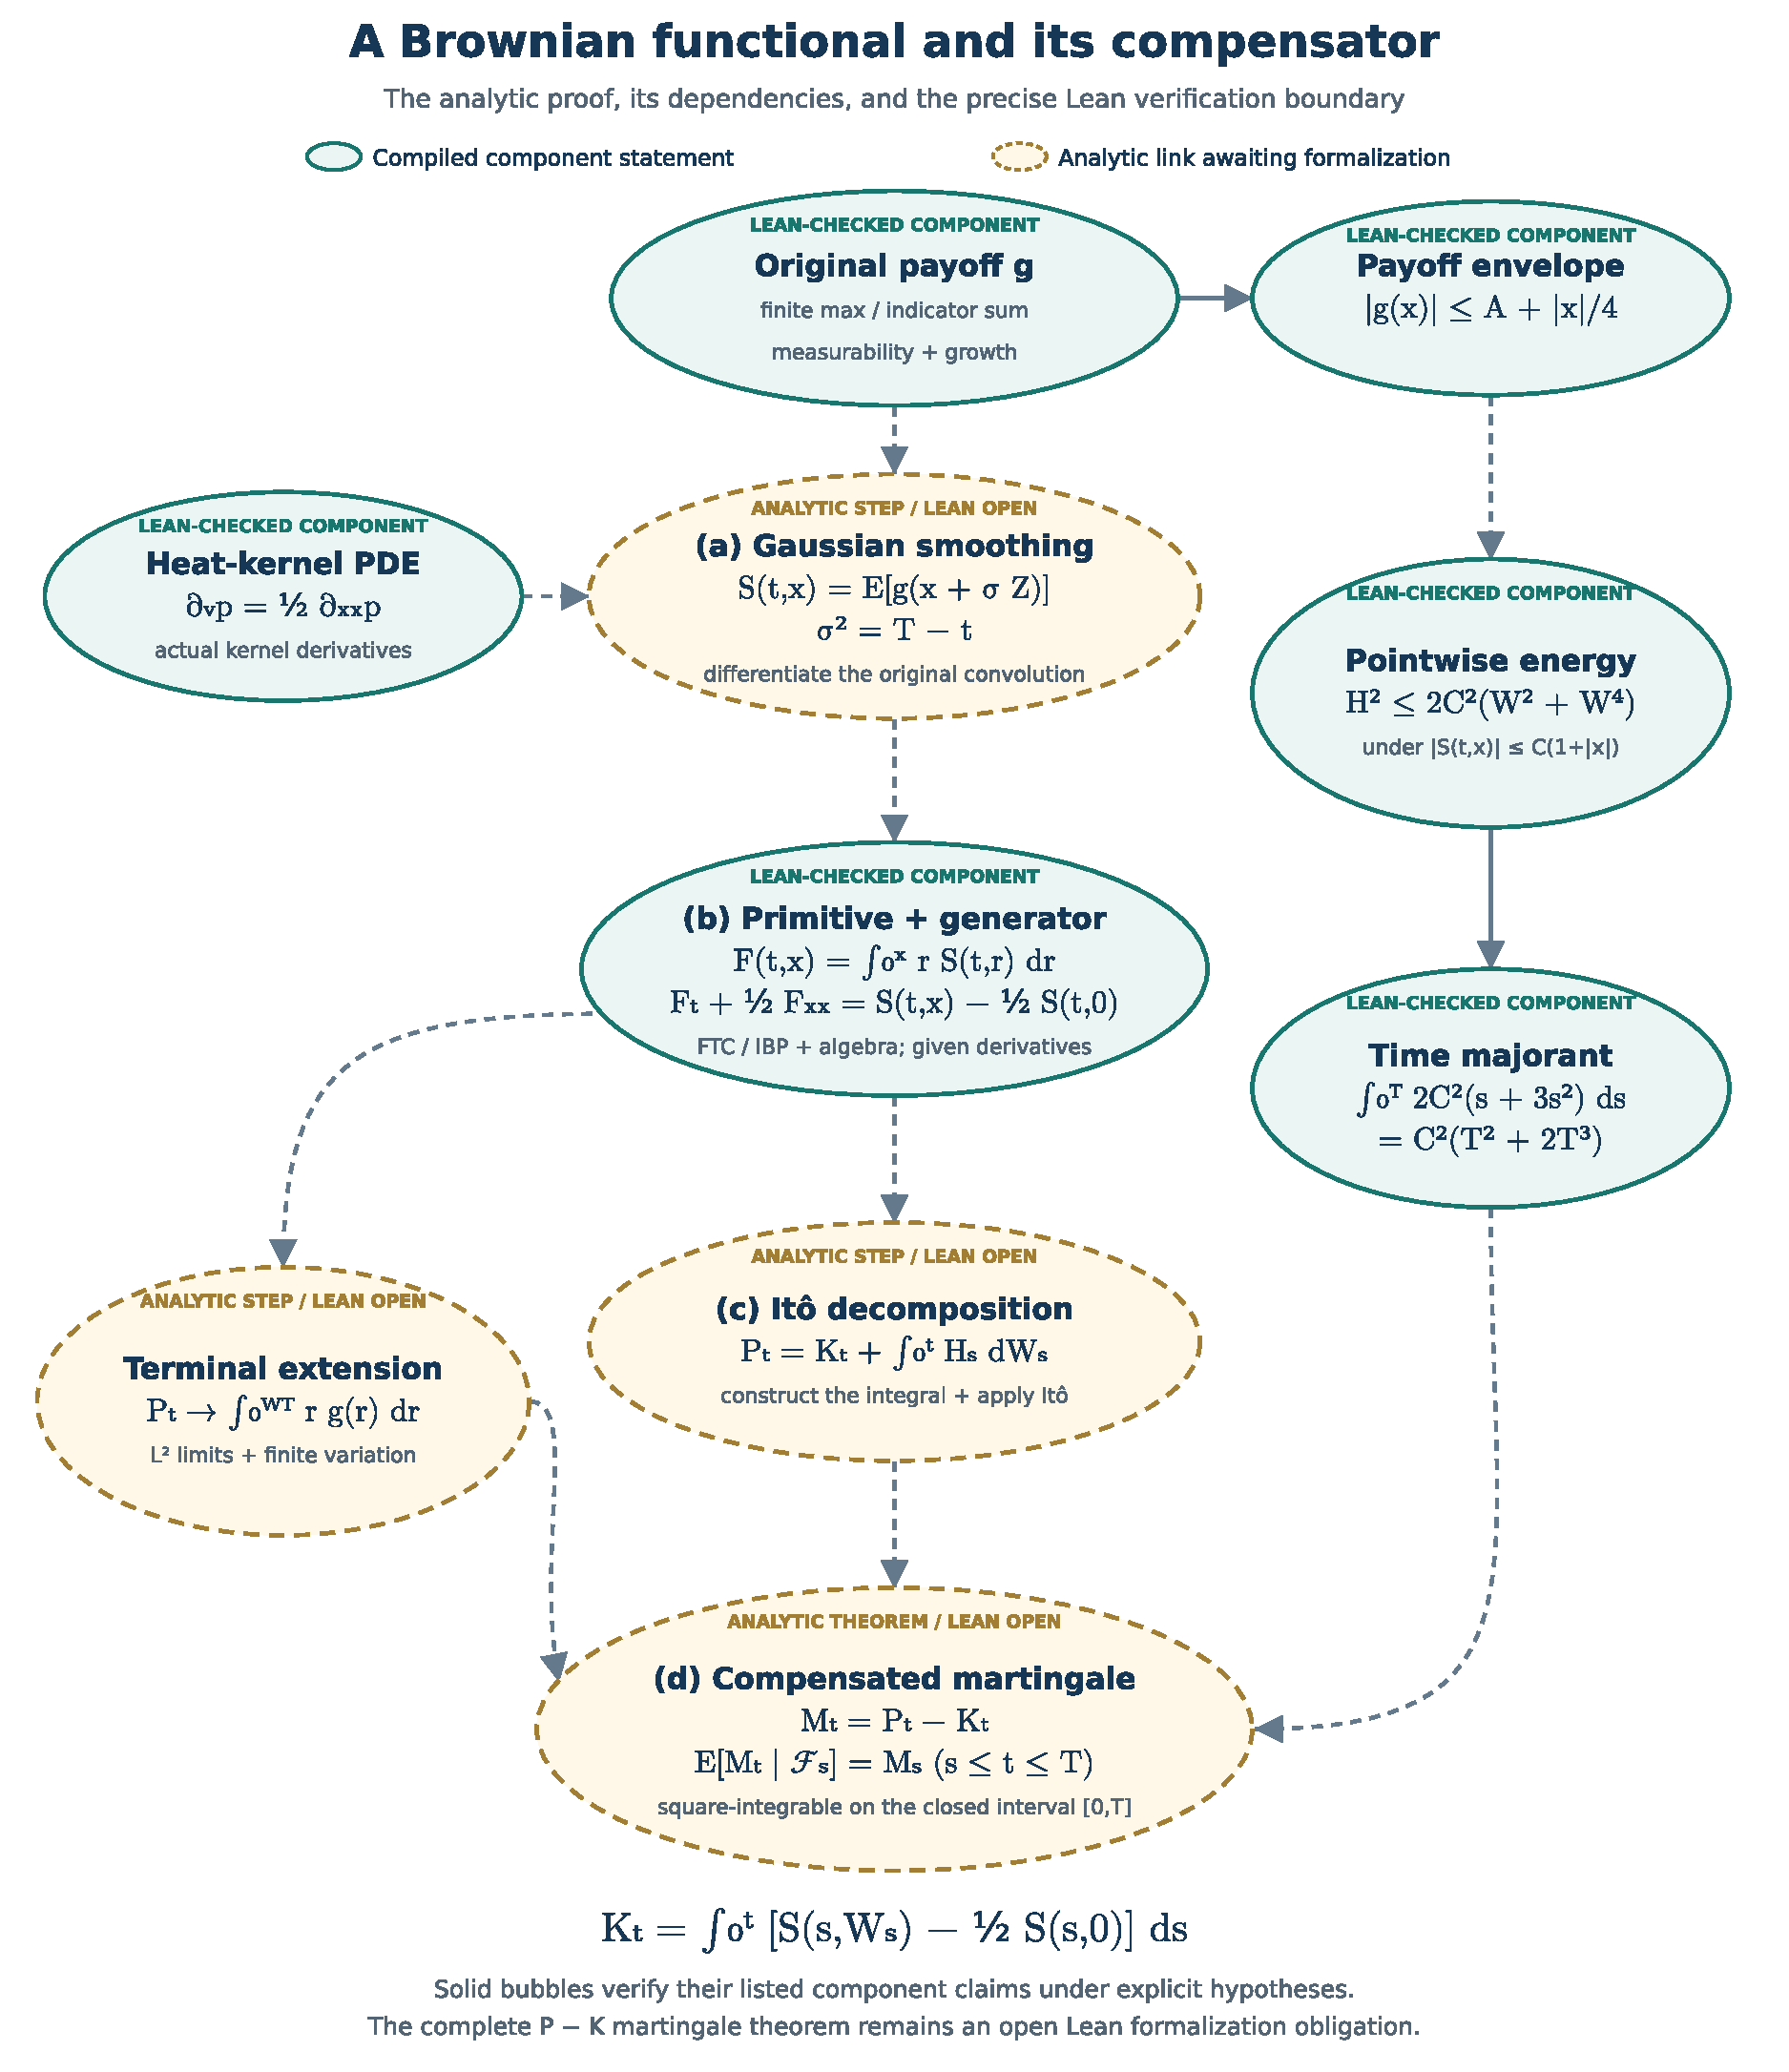
\includegraphics[width=.91\linewidth]{figures/proof_map.pdf}
\caption{Proof idea bubble map. The vector artwork is generated directly from \texttt{proof\_map.svg}; text and curves remain vector graphics in this PDF. Teal solid bubbles identify compiled component statements. Amber dashed bubbles identify analytic steps with remaining formalization work.}
\label{fig:proofmap}
\end{figure}
\clearpage

\begingroup\fontsize{10.1}{12.3}\selectfont
\section{Numerical experiments for the recorded payoff}
\subsection*{Design and interpretation}
The recorded problem allows arbitrary parameters. We choose the illustrative values
\[
T=1,\qquad n=3,\qquad(a_1,a_2,a_3)=(-0.75,0,0.85).
\]
These are example parameters, rather than fitted data. The numerical code uses \SamplePaths\ independent Brownian paths, \FineSteps\ fine time steps, seed \RandomSeed, and nested coarser grids with 64, 128, 256, 512, 1024 and 2048 steps. All figures and CSV tables are generated by \texttt{numerics.py}.

The Gaussian formula \eqref{eq:Sexplicit} evaluates $S$. Spatial antiderivatives evaluate $P$ without spatial grid interpolation. The finite-variation integral uses the composite trapezoidal rule, while the stochastic integral uses \emph{left-endpoint} predictable sums. Writing $h=T/N$, the discrete residual is
\[
R_N=P_T-K_T^{(N)}-\sum_{j=0}^{N-1}W_{t_j}S(t_j,W_{t_j})(W_{t_{j+1}}-W_{t_j}).
\]
Comparing the same nested sample paths separates discretization effects from a change of random sample.

\subsection*{Closed spatial antiderivatives}
Let
\[
I_0(y)=y\Phi(y)+\varphi(y),\qquad
I_1(y)=\tfrac12[(y^2-1)\Phi(y)+y\varphi(y)].
\]
For $y=(r+a)/\sigma$, an antiderivative of $rH_\sigma(a+r)$ is
\begin{equation}
J_a(r)=\frac{\sigma^3}{3}[y^3\Phi(y)+(y^2-1)\varphi(y)]
-\frac{a\sigma^2}{2}[(y^2+1)\Phi(y)+y\varphi(y)].
\end{equation}
For $y=(c-r)/\sigma$, an antiderivative of $r\Phi((c-r)/\sigma)$ is
\begin{equation}
L_c(r)=-c\sigma I_0(y)+\sigma^2I_1(y).
\end{equation}
Evaluating each primitive between $0$ and $x$ gives
\begin{equation}
F(t,x)=-\frac1{4n}\sum_i[J_{a_i}(x)-J_{a_i}(0)]
+\frac D2x^2-\frac1{4n^2}\sum_{i,j}[L_{c_{ij}}(x)-L_{c_{ij}}(0)].
\end{equation}
At $t=T$, use $J_a(r)=(r+a)_+^3/3-a(r+a)_+^2/2$ and $L_c(r)=\min(r,c)^2/2$, evaluating the same endpoint differences. Direct adaptive quadrature independently checks these formulas over both positive and negative spatial intervals.

\subsection*{Computed results}
\begin{center}
\begin{tabularx}{\linewidth}{@{}Xr@{}}\toprule
Quantity & Result\\\midrule
Maximum error: closed $S$ versus Gaussian quadrature & \SemigroupError\\
Maximum error: closed $F$ versus spatial quadrature & \PrimitiveError\\
Deterministic quadrature: $\E P_T$ & \ExpectedP\\
Deterministic quadrature: $\E K_T$ & \ExpectedK\\
Monte Carlo: $\E M_T$ estimate & \MeanM\\
Monte Carlo: standard error of that estimate & \SEMeanM\\
Nested-grid RMS residual, 64 steps & \CoarseError\\
Nested-grid RMS residual, 2048 steps & \FineError\\
Fitted log--log slope of the residual & \ConvergenceSlope\\
Finite-difference PDE RMS residual, $h=0.00125$ & \PDEError\\
Adaptive spatial/time quadrature: $\E\int_0^TH_s^2\dd s$ & \EnergyAdaptive\\
Proved conservative upper bound $C^2(T^2+2T^3)$ & \EnergyBound\\\bottomrule
\end{tabularx}
\end{center}
\endgroup
\clearpage
\begin{figure}[p]\centering
\includegraphics[width=.96\linewidth]{figures/01_payoff_and_semigroup.pdf}
\caption{The original positive-part/indicator payoff and its Gaussian smoothing at four times. The sharp terminal structure is retained.}
\vspace{8pt}
\includegraphics[width=\linewidth]{figures/02_heat_and_drift.pdf}
\caption{Space--time values of the heat solution and the compensator density $b(t,x)=S(t,x)-S(t,0)/2$. The horizontal and vertical scales agree across the two panels.}
\end{figure}
\clearpage
\begin{figure}[p]\centering
\includegraphics[width=.85\linewidth]{figures/03_path_decomposition.pdf}
\caption{One reproducible Brownian path. The lower panel measures the residual between the functional decomposition and the left-point stochastic sum.}
\vspace{6pt}
\includegraphics[width=\linewidth]{figures/04_martingale_diagnostics.pdf}
\caption{Unconditional and coarse conditional mean checks. Error bars show 1.96 Monte Carlo standard errors. Conditioning bins use only the midpoint state, a restricted subset of midpoint information.}
\end{figure}
\clearpage
\begin{figure}[p]\centering
\includegraphics[width=\linewidth]{figures/05_numerical_convergence.pdf}
\caption{Nested stochastic discretizations and an independent centered finite-difference check of the backward heat equation. The $h^{1/2}$ line is a reference scale.}
\vspace{8pt}
\includegraphics[width=\linewidth]{figures/06_energy_and_terminal_law.pdf}
\caption{Finite stochastic-integral energy and the conservative polynomial bound. The terminal martingale law is asymmetric; the martingale assertion concerns conditional means.}
\end{figure}
\clearpage

\section{Lean verification ledger and reproducibility}
\textbf{Compiler.} Lean 4.36.0; Mathlib tag \texttt{v4.36.0}, commit
\texttt{fc4f59e577feb1a4956671bc04ac18aaaf8cd842}.
The exact source files, compiler output, theorem-name registry, checksums, and axiom reports accompany the package. Every included theorem is compiled; each theorem's hypotheses remain visible in its statement. No new axioms or proof placeholders are introduced by these files.

\begin{center}
\small
\begin{tabularx}{\linewidth}{@{}p{.24\linewidth}Xp{.18\linewidth}@{}}\toprule
Component & Precisely verified statement & Formal status\\\midrule
Original payoff & Indicator equivalence; Borel measurability; linear-growth bound for the actual finite double sum & Compiled\\
Heat kernel & Actual first and second derivatives and forward/backward heat equations of the logarithmic Gaussian kernel & Compiled\\
Spatial primitive & Actual interval-integral first/second derivatives and weighted integration by parts under stated smoothness hypotheses & Compiled\\
Compensator coefficient & Exact generator cancellation retaining the spatial lower-endpoint term & Compiled\\
Integrability ingredients & Pointwise energy bound; actual time integral of the polynomial majorant; Brownian finite moments; actual terminal payoff in $L^p$ & Compiled\\
Conditional payoff & Martingale formed by conditional expectations of the actual terminal payoff & Compiled\\
Quadratic benchmark & Gaussian convolution and backward heat equation for $g(x)=x^2$ & Compiled; separate test\\\midrule
Original heat convolution & Differentiate the original payoff convolution with all domination hypotheses discharged, and identify it with the explicit smoothing formula & Open\\
Stochastic integration & Construct the predictable $L^2$ It\^o integral and its isometry in Lean & Open\\
Functional decomposition & Apply a proved It\^o formula to this $F$ and identify $P-K$ with the integral & Open\\
Closed-interval conclusion & Formal terminal $L^2$ limit, predictable finite variation, and the full $P-K$ martingale theorem on $[0,T]$ & Open\\\bottomrule
\end{tabularx}
\end{center}
The conditional-payoff theorem in the compiled module concerns $\E[g(W_T)\mid\F_t]$. The analytic identity \eqref{eq:StCE} and the compensator identity \eqref{eq:main} are separate statements. The axiom audit and a successful compiler run are evidence for the listed theorem statements; they do not extend that coverage to the open rows.

\textbf{Reproduction.} Install the pinned Lean toolchain, run \texttt{verify.sh} against the pinned Mathlib checkout, install \texttt{requirements.txt}, execute \texttt{numerics.py}, and compile \texttt{paper.tex} twice with XeLaTeX. The README gives exact commands and source hashes. Figures have embedded English labels and use STIX text/math; the paper uses Latin Modern Roman and Latin Modern Math with embedded fonts.

\subsection*{Public source and reproducible Lean verification}
The published source is fixed at repository commit
\begin{center}\texttt{73a1d2ff4f3125264fe3d2e9d1daa013fd31582e}.\end{center}
Repository: \url{https://github.com/Eliguli712/brownian_motion}.\\
Permanent source: \href{https://github.com/Eliguli712/brownian_motion/blob/73a1d2ff4f3125264fe3d2e9d1daa013fd31582e/compensator/Brownian_Compensator_Verified_Components.lean}{\texttt{Brownian\_Compensator\_Verified\_Components.lean}}.

The linked \href{https://github.com/Eliguli712/brownian_motion/actions/runs/45158953034}{Actions run} completed successfully for this source commit. It installs Lean 4.36.0, checks out the exact Mathlib commit, compiles all 39 included statements with warnings treated as errors, and prints their axiom dependencies. Its job name is \emph{Compile and audit 39 component theorems}.

To reproduce the same verification, install the Lean toolchain and run:
\begin{small}
\begin{verbatim}
elan toolchain install leanprover/lean4:v4.36.0
git clone https://github.com/Eliguli712/brownian_motion.git
cd brownian_motion
git checkout 73a1d2ff4f3125264fe3d2e9d1daa013fd31582e
git clone https://github.com/leanprover-community/mathlib4.git .mathlib
git -C .mathlib checkout fc4f59e577feb1a4956671bc04ac18aaaf8cd842
cd .mathlib
lake exe cache get Mathlib.Probability.BrownianMotion.Basic \
  Mathlib.Probability.Martingale.Basic \
  Mathlib.MeasureTheory.Integral.IntervalIntegral.IntegrationByParts \
  Mathlib.Analysis.SpecialFunctions.Integrals.Basic \
  Mathlib.Analysis.SpecialFunctions.Log.Deriv \
  Mathlib.Analysis.SpecialFunctions.ExpDeriv Mathlib.Tactic
cd ..
bash compensator/verify.sh "$PWD/.mathlib"
\end{verbatim}
\end{small}
The script checks the Mathlib revision before invoking Lean. A successful component-verification run certifies the statements listed in the ledger. The complete $P-K$ martingale theorem retains the open obligations listed above.

\textbf{Source record.} The recovered four-page solution supplies the recorded problem. The new proof, code and numerical experiments are delivered as separate files. The original recovered PDF remains available as the source record. The formalization builds on the source files \path{Mathlib/Probability/BrownianMotion/Basic.lean}, \path{Mathlib/Probability/Martingale/Basic.lean}, and the interval-integral calculus modules at the pinned revision.

\end{document}
